\chapter{Introduction}
\label{ch:introduction}

\section{Motivation}
  Recent interest in advanced and next-generation nuclear power reactor designs
  has encouraged further development of simulations for these reactors. A class
  of advanced nuclear power reactors meriting research since the dawn 
  of nuclear engineering is the Sodium-cooled Fast Reactor (SFR) which operate
  with liquid sodium coolant and operate with predominantly high-energy 
  (``fast'') neutrons in the fission reaction. Since early development of SFRs 
  such as the Experimental
  Breeder Reactor I (EBR-I) in 1951 and Fermi 1 in 1956, there have been
  significant innovations in both nuclear modeling and computational methods. As
  development of SFRs is revisited in the form of the Versatile Test Reactor
  (VTR) at Idaho National Laboratory (INL), these innovations in simulation can
  be used to simulate SFRs with modern best practices.
  Though this discussion has focused on reactors designed with sodium coolant,
  these methods can easily be used for reactors with lead or molten salt
  coolant.

  Nuclear reactor simulations are inherently multi-physics simulations. For
  example, neutron reaction probabilities are described by cross-sections.
  Neutron cross-sections are dependent on material temperatures and densities,
  both of which vary over the operating range of a nuclear power reactor. As
  reactor power changes, material temperatures and densities change, therefore
  cross-sections change and affect the reactor power. The multi-physics nature
  of the reactor necessitate a simulation of the power distribution within the
  reactor as well as all physical effects which will be modeled. In this
  work, the mulitgroup neutron diffusion equation is used to describe the 
  reactor power distribution as in \chref{ch:neutronDiffusion}. Multi-physics 
  effects are described by heat conduction and heat convection models as in
  \chref{ch:thermalHydraulics} as well as a thermal expansion model as in
  \chref{ch:thermalExpansion}.

  Ultimately, this simulation will model the steady-state behavior of SFRs using
  modern methods. By employing a modern solution method to the neutron diffusion
  equation in the form of the Finite Element Method (FEM), the simulation can
  take advantage of developments in numerical methods including the solution of
  linear systems. Additionally, the simulation allows for the incorporation of
  generalized multi-physics effects whereas current state-of-the-art simulations
  require data processing and manual iteration to simulate multi-physics 
  effects. The final simulation is designed to simulate an operating SFR.

\section{Geometry Description}
  \label{sec:geometry_description}
  Operating with fast neutrons decreases reaction probabilities. To compensate
  for this fact, SFRs are typically designed with hexagonal,
  triangularly pitched, fuel assemblies to maximize the fuel packing and
  increase the fuel density. An example of an SFR with hexagonal geometry as
  simulated in this method is shown in \fref{fig:reactor_materials}.
  A typical hexagonal fuel assembly is displayed in \fref{fig:prism_hex}.
  This geometry is used to describe material properties in the form of 
  cross-sections as well as to describe coolant flow geometries. Dimensions of 
  assemblies are measured at room temperature and will later be expanded 
  according to the thermal expansion model in \chref{ch:thermalExpansion}.
  
  \begin{figure}
    \centering
    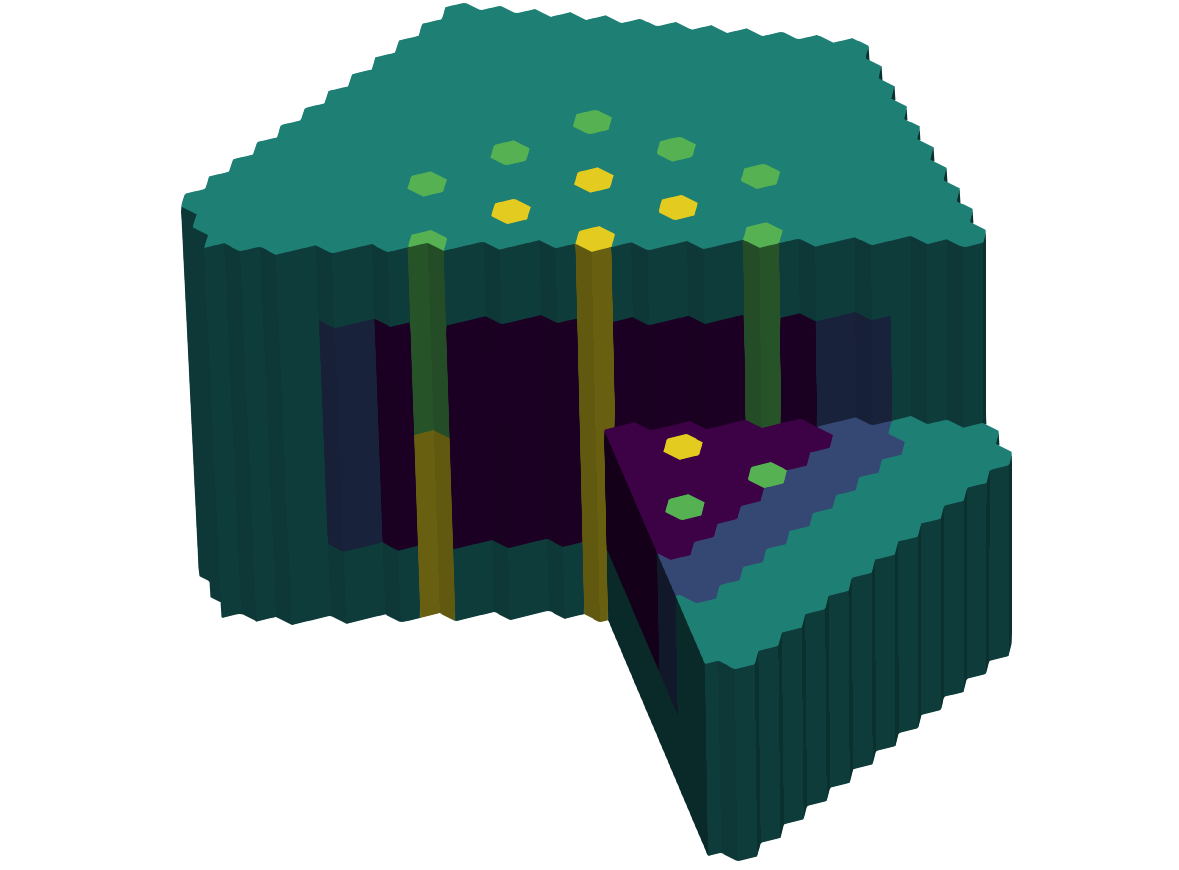
\includegraphics[width=\textwidth]{reactor_materials}
    \caption{Example of Sodium-cooled Fast Reactor based on MONJU.}
    \label{fig:reactor_materials}
  \end{figure}

  \begin{figure}
    \centering
    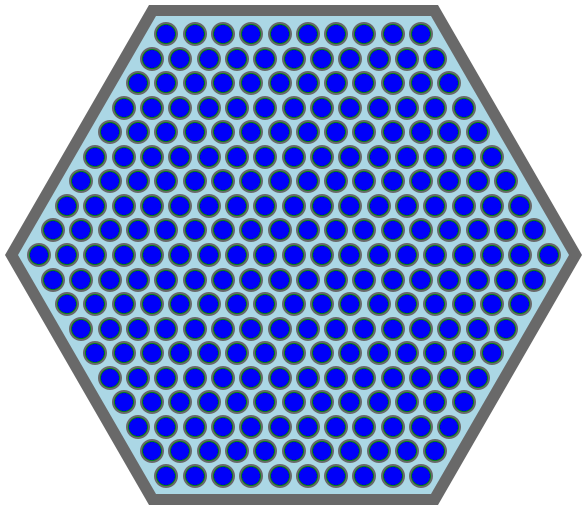
\includegraphics[width=0.5\textwidth]{prism_hex}
    \caption{Example of Sodium-cooled Fast Reactor Fuel Assembly.}
    \label{fig:prism_hex}
  \end{figure}

  In a cross sectional representation of a hexagonal assembly, dimensions are 
  shown in \fref{fig:prism_hex}. 
  Note the individual material pins are cylindrical and are then accumulated
  into a hexagonal assembly. The basic geometry is a fuel material within
  stainless steel cladding. The gap between the fuel and cladding is filled by
  sodium bond to improve thermal conductivity across the gap. Then the pin is
  wrapped by a steel wire to ensure separation between pins that will allow for
  coolant flow. The wire wrap also serves to encourage the mixture of coolant
  within the assembly. (Note: wire wrap is omitted from \fref{fig:prism_hex}.) 
  Many pins are then assembled into an assembly and surrounded by a hexagonal 
  can made of steel. This can aids in structural stability and prohibits 
  cross-flow between assemblies. 

  The dimensions within a single pin are shown in \fref{fig:pin_model} and the
  dimensions within a hexagonal assembly can are shown in \fref{fig:hex_can}. In
  \fref{fig:hex_can}, $T\!h_{Box}$ is the thickness of the assembly box,
  $F\!2\!F$ is the flat-to-flat measurement of the outside of the hexagonal can,
  and Pitch is the distance between the center of two pins.
  Using the geometry described in 
  these figures, the material cross-sectional areas are calculated according to 
  the given formulae where $N_{pin}$ is the number of pins in the assembly.
  \begin{align}
    \label{eq:afrac_first}
    A_{total} &= \frac{\sqrt{3}}{2} F\!2\!F^2 \\
    A_{can} &= A_{total} - 
      \frac{\sqrt{3}}{2} \left(  F\!2\!F - 2 \, T\!h_{Box} \right) \\
    A_{wrap} &= N_{pin} \frac{\pi}{4} D_{wrap}^2 \\
    A_{clad} &= N_{pin} \pi (R_C^2 - R_B^2) \\
    A_{bond} &= N_{pin} \pi (R_B^2 - R_F^2) \\
    A_{fuel} &= N_{pin} \pi R_F^2 \\
    \label{eq:afrac_last}
    A_{cool} &= A_{total} - A_{can} - A_{wrap} - A_{clad} - A_{bond} - A_{fuel}
  \end{align}
  Calculating the areas as above allows for calculation of cross-sectional area
  fractions. Assuming constant dimensions in the axial
  direction, these area fractions are equivalent to volume fractions and are
  useful for neutron cross-section calculations. Additionally, these formulae
  allow for thermal expansion as the liquid sodium in the bond and
  the liquid coolant are allowed to vary to allow for the expansion of other 
  materials.

  \begin{figure}
    \centering
    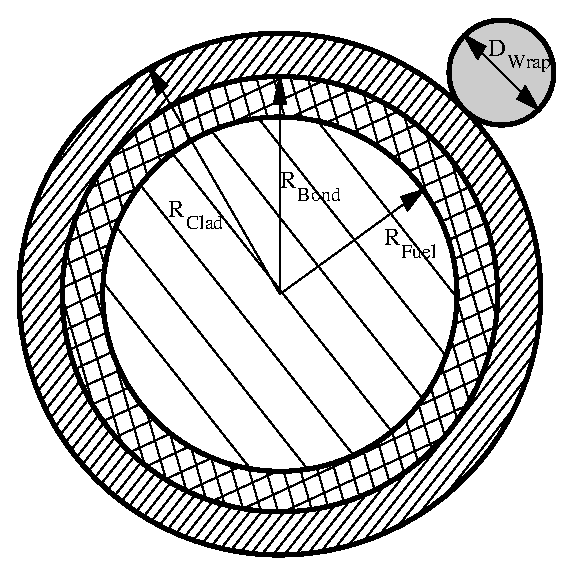
\includegraphics[width=0.5\textwidth]{pin_model}
    \caption{Dimensions of Thermal Hydraulic Pin Model.}
    \label{fig:pin_model}
  \end{figure}

  \begin{figure}
    \centering
    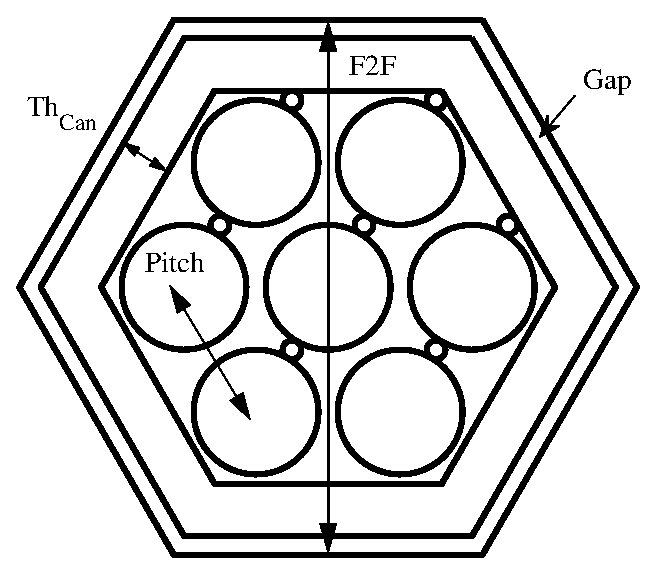
\includegraphics[width=0.5\textwidth]{hex_can}
    \caption{Dimensions of Hexagonal Can.}
    \label{fig:hex_can}
  \end{figure}

\section{Cross-Section Treatment}
  \label{sec:cross_section_treatment}
  Reactor materials are ``smeared'' into homogeneous regions. This assumption is 
  common to fas reactors because of the relatively large neutron mean-free-paths
  compared to the scale of material dimensions. 
  The natural choice for these homogenized regions are the hexagonal
  assemblies themselves. Materials are permitted to be heterogeneous axially but
  are homogenized in the radial direction within each assembly. For a number
  density $N_i$ within region $i$, the homogenized number density is
  \begin{equation}
    \label{eq:homogenized_nden}
    \overline{N} = \frac{\sum_{i = 1}^{N_{reg}} N_i \, V_i}
      {\sum_{i=1}^{N_{reg}} V_i}
  \end{equation}
  where $V_i$ is the volume of the region and $N_{reg}$ is the number of
  regions. For this simulation, ${N_{reg}=4}$ representing fuel, bond, coolant,
  and steel. Steel material includes cladding, wire wrap, and the assembly can.
  \eref{eq:homogenized_nden} is then evaluated using the areas in
  \eref{eq:afrac_first} through \eref{eq:afrac_last}. Assuming the same height
  in each region, area fractions can be translated to volume fractions to use in
  the formula.

  For benchmark and analytic problems, cross-sections are simply given as
  constants for the problem. Realistic reactor simulations require
  cross-sections generated from preliminary calculations. In this
  work, multigroup microscopic cross-sections are generated using 
  \mcc \cite{mcc}.
  The cross-section generator uses 2,082 fine energy groups to collapse down
  to an arbitrary number of energy-groups. For this simulation, the
  recommended and default 33-group energy structure is used. \mcc 
  collapses the geometry to an infinite homogeneous medium and isotopic number
  densities are calculated and input using \eref{eq:homogenized_nden}.
  Cross-sections for each assembly type are generated separately to accurately
  simulate the neutron energy spectrum within the assembly. The neutron energy
  spectrum for fissile media is generated by the media's fission spectrum. 
  Non-fissile material uses the default \isotope[238]{U} fission spectrum. 

  To capture the effect of Doppler broadening, cross-section libraries are
  generated for several different material temperatures. These libraries are
  then used during the simulation to calculate on-the-fly cross-sections as a
  function of material temperatures.
  While fuel, clad, and coolant temperatures can be related with a thermal
  hydraulic model (see \chref{ch:thermalHydraulics}, these relationships are 
  functions of reactor power and coolant mass flow rate. These parameters are
  not known before the simulation for a general reactor. Instead, a simplified
  temperature relationship is used to generate the cross-section libraries.

  In each cross-section library, the coolant is maintained at some nominal
  temperature. For this work, that temperature is $400 \units{K}$
  (note: sodium melting temperature 371 \units{K}). Maintaining the coolant
  temperature as constant in this manner is acceptable because the dominant 
  effect of temperature on the macroscopic cross-sections in the coolant is 
  the density change of the fluid, not the Doppler effect. With constant 
  coolant temperature, the fuel temperature is then varied over some range. 
  In this work, libraries are generated for average fuel temperatures
  of $400 \units{K}$, $600 \units{K}$, $900 \units{K}$, and $1200 \units{K}$.
  At each fuel temperature, the clad temperature is related as 
  \begin{equation}
    T_{clad} = \max \left\{ w \, T_{fuel}, T_{cool} \right\}
  \end{equation}
  % note: weight for T_{cool} should be 0.63 if perturbed coolant is desired
  where $w$ is a weighting factor, $T_{fuel}$ is the chosen fuel temperature
  for the library, and $T_{cool}$ is the chosen coolant temperature for the
  library. A weighting of $w=0.7$ was selected based on analysis of the ratio
  $T_{clad}/T_{fuel}$ for a representative high power channel
  within an example reactor simulation.  Temperature in non-fissile assemblies 
  is set to $T_{cool}$ during the collapse as there is no heat generation 
  modeled in these materials.

  \begin{table}
    \caption{Temperatures Selected for Cross-Section Libraries.}
    \label{tab:xstemps}
    \begin{center}
      \begin{tabular}{lll}
        \toprule
        $T_{cool} \units{K}$ & $T_{clad} \units{K}$ & $T_{fuel} \units{K}$ \\
        \midrule
        400 & 400 & 400  \\
        400 & 420 & 600  \\
        400 & 630 & 900  \\
        400 & 840 & 1200 \\
        \bottomrule
      \end{tabular}
    \end{center}
  \end{table}

  Ultimately, the cross-sections are accumulated as four separate libraries at
  temperatures given in \tref{tab:xstemps}. Then, these libraries are used to
  calculate on-the-fly cross-sections during the simulation.
  With given microscopic cross sections calculated by \mcc, macroscopic cross
  sections are calculated by homogenizing microscopic with number densities
  $N_{i,j}$ for isotope ${j=1,2,\ldots,N_{iso}}$ in region
  ${i=1,2,\ldots,N_{reg}}$.  For the $x$ reaction type, the 
  macroscopic cross-section is defined as
  \begin{equation}
    \Sigma_{x,g} = \frac{\sum_{i=1}^{N_{reg}} \sum_{j=1}^{N_{iso}} V_i N_{j} 
      \sigma_{x,g,i}} {\sum_{i=1}^{N_{reg}}V_i}
  \end{equation}
  again using the area formulae from \eref{eq:afrac_first} through
  \eref{eq:afrac_last} to calcualte the volume fractions of each regin.
  Finally, the homogenized transport cross section is used to calculate the 
  diffusion coefficient.
  \begin{equation}
    D_g = \frac{1}{3 \Sigma_{tr,g}}
  \end{equation}

\section{Thesis Organization}
  In \chref{ch:neutronDiffusion}, the derivation of the Finite Element Method is
  presented for triangular and wedge elements. The resulting eigenvalue problem
  is then solved using the power method. Results from the diffusion solution are
  verified in two-dimension and three-dimension problems with both analytic and
  benchmark solutions. These verification problems for the neutron diffusion
  equation are presented in \chref{ch:diffusionResults}.

  \chref{ch:thermalHydraulics} presents the formulation of axial heat convection
  and radial heat conduction models for a typical SFR. These models are used to
  calculate material temperatures and update cross-sections for the simulation.
  Results of the numerical model is compared to analytical models and example
  system temperatures are shown.

  The materials are expanded according to thermal expansion behavior as
  described in \chref{ch:thermalExpansion}. This model allows for the realistic
  simulation of an SFR and results of the simulation of a model SFR are presented
  in \chref{ch:coupledResults}. Finally, \chref{ch:conclusions} presents a 
  summary and the conclusions of this research. Additionally, recommendations 
  for further research are included.

